\part{Información General}

\chapter{Presentación}

Las V Jornadas de Usuarios de R tendrán lugar en el
\href{http://www.zaragoza.es/ciudad/idezar/detalle_Centro?id=5105}{Etopia-Centro
  de Arte y Tecnología de Zaragoza}, los días 12 y 13 de diciembre de
2013. Etopia es un centro de creatividad, innovación y emprendimiento,
16.000 m2 para el trabajo colaborativo, la búsqueda de nuevos caminos
y para aprender haciendo y compartiendo. Forma parte de la
\href{http://www.zaragoza.es/ciudad/sectores/tecnologia/milladigital.htm}{Milla
  Digital de Zaragoza}, promovida por el
\href{http://www.zaragoza.es/ciudad/sectores/tecnologia/}{Área de
  Tecnología del ayuntamiento de Zaragoza}.

Las jornadas, como no podría ser de otra forma, van a incluir trabajos
de todos los ámbitos y están abiertas tanto a usuarios como a
entusiastas de R independientemente de su área de interés. Los
objetivos para estas jornadas serán los mismos que para las anteriores
que tan buenos resultados obtuvieron. Estos objetivos incluyen:

\begin{itemize}
\item Proporcionar un punto de encuentro a los usuarios de R 
\item Fomentar la colaboración entre ellos en un ambiente multidisciplinar 
\item Divulgar el conocimiento del lenguaje y sus posibilidades 
\item Promover el uso de R 
\end{itemize}

Usuarios y entusiastas de R de todos los ámbitos —universidad,
institutos de investigación, administraciones públicas, empresa
privada— están invitados a participar en las V Jornadas y compartir
con la comunidad aplicaciones y ejemplos interesantes que reflejen la
madurez de R y la diversidad de los problemas y campos en los que
viene utilizándose con éxito. Existen las siguientes modalidades de
participación:
\begin{itemize}
\item Comunicaciones orales de 15 minutos seguidas de una discusión de
  5 minutos (la decisión sobre la duración podría sufrir
  modificaciones en función del número final de ellas).

\item Presentaciones breves de 5 minutos, donde el ponente expone en
  tres diapositivas (número orientativo) de forma breve y concisa,
  quién es/son, qué ha/n hecho, y qué resultados y conclusiones se
  extraen de ello que puedan ser de interés para otras personas.

\item Talleres de 2 horas aproximadamente, donde se explican paquetes,
  procedimientos, y programas de R.  En esta edición, además de las
  ponencias invitadas, las presentaciones orales y los talleres, se
  llevarán a cabo presentaciones breves donde el ponente expondrá de
  forma concisa los resultados y conclusiones de alguna investigación
  llevada a cabo con R que puedan ser de interés para otros colegas.
\end{itemize}

Desde el comité organizador nos gustaría destacar la excelente labor
llevada a cabo por el comité científico, a los ponentes de los
talleres y a todos los asistentes y patrocinadores que han permitido 
confeccionar el programa que a continuación detallamos y esperamos que 
sea de vuestro interés.

Esperamos que las jornadas resulten lo más provechosas posibles y que
disfrutéis de una confortable estancia en Zaragoza.


\chapter{Información útil}

\section{Ubicación de las jornadas}

Las jornadas se celebrarań en el Centro de Arte y Tecnología 
\href{http://www.zaragoza.es/ciudad/idezar/detalle_Centro?id=5105}{CAT-ETOPIA}
que  el Ayuntamiento de Zaragoza ha desarrollado en la llamada 
\href{http://www.milladigital.es/espanol/home.php}{Milla Digital}. 

\begin{center}

\includegraphics[width=0.6\textwidth]{Logos/logoMillaAyZgz.png}
\end{center}

El C.A.T. está situado prácticamente en el centro de la Milla Digital, 
justo enfrente de la Estación de Delicias, con la cual se encuentra 
comunicado mediante un puente peatonal conocido como la 
\href{http://www.puentemania.com/692}{Pasarela Delicias}.  Este área de 
Zaragoza se encuentra comunicado con el centro de la ciduad (Puerta del 
Carmen y Plaza del Paraiso) mediante las lineas de autobuses
\href{http://www.urbanosdezaragoza.es/frm_verdescarga.php?ref=175}{34 y 52},
también pueden resultar de interés las lineas circulares
\href{http://www.urbanosdezaragoza.es/frm_verdescarga.php?ref=175}{Ci1 y Ci2}.

\begin{center} 
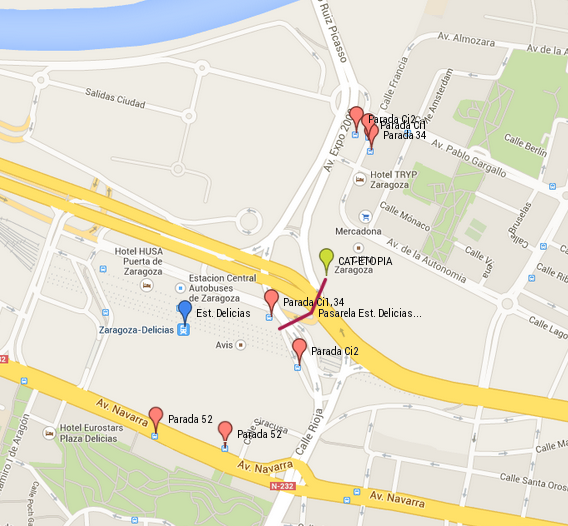
\includegraphics[width=0.6\textwidth]{Logos/mapaParadas.png}
\end{center}



Las comunicaciones orales y breves se llevarán a cabo en el auditorio 
William J. Mitchell del CAT-ETOPIA. Para acceder al edificio cada 
participante se deberá identificar en recepción donde disponen de una 
lista con todos los asistentes.


\section{Talleres}

Los participantes a los talleres deben traer su propio ordenador portátil 
con las herramientas y en las condiciones que indiquen los responsables de 
los talleres. La inscripción a los talleres se realizará en el momento de 
la entrega de material, en el momento de la recepción de los participantes. 
Dado el limitado número de plazas, se reservará plaza por orden de inscripción. 
Los talleres se desarrollarán en las aulas de que dispone el CAT-ETOPIA 
para laboratorios audiovisuales y meetings.


\section{Certificados}

Los certificados relativos a la asistencia y participación en las jornadas
se entregarán durante la celebración de las mismas.

% enviarán por correo electrónico una vez pasadas
% las Jornadas.  

\section{Material}

Todo el material estará disponible a través de la página web de las Jornadas 
\href{http://r-es.org/V+Jornadas}. 



\chapter{Comité organizador}

\begin{itemize}

\item \href{http://www.datanalytics.com}{C. Gil Bellosta}
  (coordinador, Datanalytics)
\item \href{http://www.scien-analytics.com}{Sergio Jiménez} (Scien Analytics)
\item Luis Mariano Esteban (Universidad de Zaragoza)
\item \href{http://www.scien-analytics.com}{Rubén Moreno Ruíz} (Scien Analytics)
\item \href{[http://www.scien-analytics.com}{Miguel Ángel Luzón} (Scien Analytics)
\item Jorge Ojeda (Universidad de Zaragoza)
\item \href{http://ueb.vhir.org|Vall d'Hebron Research Institute}{Xavier de Pedro Puente} (Vall d' Hebron Research Institute)
\item  Emilio Torres Manzanera (Universidad de Oviedo)
\end{itemize}

\chapter{Comité científico}


\begin{itemize}

\item Sandra Barragán (Universidad de Valladolid)
\item Ramón Díaz-Uriarte (Universidad Autónoma de Madrid)
\item Juan Ramon González (Centro de Investigación en Epidemiología Ambiental)
\item \href{http://oscarperpinan.github.io}{Oscar
    Perpiñán}(Universidad Politécnica de Madrid)
\item Miguel Angel Rodríquez (coordinador, Xunta de Galicia)
\item Isaac Subirana (Instituto Hospital del Mar de Investigaciones Médicas)
\item Joan Vila (Instituto Hospital del Mar de Investigaciones Médicas)
\item \href{http://www.ottofwagner.es}{Otto F. Wagner} (Ilustre Colegio de Economistas de Madrid)

\end{itemize}


\chapter{Patrocinadores}



\begin{center}


\includegraphics[width=0.33\textwidth]{Logos/logoMillaAyZgz.png}
\hspace{1cm}


\includegraphics[width=0.33\textwidth]{Logos/logoEtopia.jpg}
\hspace{1cm}


\includegraphics[width=0.33\textwidth]{Logos/logoScien.png}
\hspace{1cm}


\includegraphics[width=0.33\textwidth]{Logos/logoComRHisp.png}
\vspace{1cm}


\includegraphics[width=0.33\textwidth]{Logos/logoRevolAnal}
\hspace{1cm}


\includegraphics[width=0.33\textwidth]{Logos/logoUZ.png}
\hspace{1cm}


\includegraphics[width=0.33\textwidth]{Logos/logoSynergic.png}
\vspace{1cm}


\includegraphics[width=0.33\textwidth]{Logos/logoTelefID.png}

\end{center}


\chapter{Programa}

\begin{itemize}
\item \textsc{\textbf{JUEVES 15 DE NOVIEMBRE}}
  \begin{itemize}

  \item 09:00-09:30 Acreditación y recogida de información

  \item 09:30-09:45 Inauguración oficial de las Jornadas. J.R. González.

  \item 09:45-10:30 Conferencia Inaugural.  J. Vila:
    \href{http://r-es.org/tiki-download_file.php?fileId=484}{Enseñando
      estadística: como mejorar los conocimientos utilizando R
      para la creación de prácticas individualizadas.}
  \item 10:30-12:00 Sesión de Comunicaciones (I) Moderador: G.R
    Serrano
    \begin{itemize}
    \item 10:30-10:45 C. E. Melo Funciones geoestadísticas y
      funciones de base radial en el programa R: Paquete geospt
    \item 10:45-11:00 E. L. Cano Investigación operativa
      reproducible. Aplicación a la optimización de sistemas
      energéticos
    \item 11:00-11:15 C. J. Gil MicroDatosEs: un paquete para leer
      ficheros de microdatos públicos
    \item 11:15-11:30 A. Alabert Flujo de trabajo reproducible con
      R
    \item 11:30-11:45 N. Longford A study of poverty and income
      inequality in the EU countries
    \end{itemize}
  \item 12:00-12:30 Café
 
  \item 12:30-14:00 Sesión de Comunicaciones (II) Moderador:
    A. Sánchez
    \begin{itemize}
    \item 12:30-12:45 R. Pazmiño Caracterizacion del software
      estadistico en las escuelas de estadistica del
      Ecuador. Enfoque en el software R
    \item 12:45-13:00 O. Ivina A cross-country air quality
      analysis using R

    \item Comunicaciones Breves
      \begin{itemize}
      \item 13:00-13:07 M. Sánchez Inferencia estadística para el
        equilibrio de Hardy-Weinberg en estudios de genotipado con
        Missing Data
      \item 13:07-13:15 I. Roman Representación de las Dinámicas
        de Precios Hoteleros mediante R
      \item 13:15-13:22 D. Moriña El paquete complex.surv.dat.sim
        de R: Simulación de datos de supervivencia complejos
      \item 13:22-13:30 J-L. Cañadas De Excel a html utilizando
        knitr + markdown + googleVis . Un ejemplo
      \item 13:30-13:37 B. González Programación Lineal y
        Programación Dinámica con R
      \item 13:37-13:45 A. Sanz-García Selección de variables y
        modelizado predictivo en R
      \item 13:45-13:52 F. Antoñanzas-Torres Evaluación de modelos
        paramétricos de predicción de irradiación global solar
        mediante variables meteorológicas típicas
      \item 13:52-14:00 R. Fernández Uso de métodos de
        interpolación espacial para la predicción de variables en
        entornos vitivinícolas
      \end{itemize}
    \end{itemize}

  \item 14:00-16:00 Comida
  \item 16:00-17:45 Talleres (I)
    \begin{itemize}
    \item G. R. Serrano Web scraping con R
    \item F. Carmona Informes dinámicos con LaTeX y R: utilización
      de Sweave y knitr.
    \end{itemize}

  \item 17:45-18:15 Café
  \item 18:15-20:00 Talleres (II)
    \begin{itemize}
    \item X. de Pedro Interfaces Web 2.0 para R con Tiki
    \item A. Sánchez Edición (y mucho más) potente en R con ESS
      ("Emacs Speaks Statistics")
    \end{itemize}
  \item 20:00-21:00 Asamblea Asociación “Comunidad R-Hispano”

  \item 21:30 Cena

  \end{itemize}
 

 

\item \textsc{\textbf{VIERNES 16 DE NOVIEMBRE}}

  \begin{itemize}
  \item 10:00-11:00 Sesión de Comunicaciones (III) Moderador:
    F. Carmona
    \begin{itemize}
    \item 10:00-10:15 A. Lobo R como caja de herramientas para SIG
      y Teledetección: reflexiones a partir de experiencias
    \item 10:15-10:30 V. Urrea Gales Simulación de perfiles
      genéticos de riesgo
    \item 10:30-10:45 A. Urkaregi Construcción de un Índice Global
      de Valoración
    \item 10:45-11:00 G. Estévez-Pérez kerdiest: An R Package for
      Distribution Function Estimation and Applications
    \end{itemize}

  \item 11:00-12:00 Sesión de Comunicaciones (IV) Moderador:
    Ll. Ramon
    \begin{itemize}
    \item 11:00-11:15 N. M. Villanueva seq2R: Detección de puntos
      de cambio en secuencias genómicas
    \item 11:15-11:30 J Graffelman Exploring bi-allelic genetic
      markers with the HardyWeinberg package
    \item 11:30-11:45 M. Sestelo FWDselect: Selección de variables
      en modelos de regresión
    \item 11:45-12:00 B. Santos Reducción unidimensional de 12
      items de la Escala de sobrecarga de Zarit en cuidadores de
      pacientes con demencia mediante teoría de respuesta a los
      ítems.
    \item 12:00-12:15 J. Barrera The optimal Allocation package
      for longitudinal studies design with time-varying esposure
    \end{itemize}
  	 
  \item 12:15-12:45 Café

  \item 12:45-14:30 Talleres (III)
    \begin{itemize}
    \item A. Karatzoglou Machine learning in R
    \end{itemize}


  \item 14:30-16:15 Comida
  \item 16:15-18:00 Talleres (IV)
    \begin{itemize}
    \item A. Ruiz Introducción a las Reference Classes
      (programación orientada a objetos en R)
    \item Ll. Ramon, R. Borras y A. Vall Introducción práctica a
      la librería ggplot2 y su integración con ggmap
    \end{itemize}
  \item 18:00-18:30 Café

  \item 18:30-19:00 Clausura Oficial de las IV Jornadas

  \end{itemize}
\end{itemize}




